%  Latex Version of MADCOW paper with Jay Ulfelder, Shahryar Minhas, and MDW
% 25 August 2014 version
\documentclass[pdftex,12pt,fullpage,oneside]{amsart}
\usepackage[top=1in,bottom=1in,left=1in,right=1in]{geometry}
\usepackage{setspace}

\usepackage[pdftex, hyperfootnotes=false, colorlinks=true, citecolor=black, linkcolor=black, urlcolor=black, breaklinks=true]{hyperref}
\hypersetup{%
    pdftitle={MADCOW},
    pdfauthor={Shahryar Minhas, Jay Ulfelder, Michael D. Ward},
    bookmarksnumbered=true,
    citebordercolor={1 0 0},
    }
% change date format
\usepackage{datetime}
\newdateformat{mydate}{\THEDAY~\monthname[\THEMONTH] \THEYEAR}
% better citation, set punctuation.
\usepackage{natbib}
\bibpunct{(}{)}{,}{a}{}{,}
\usepackage{mathptmx}	% Times serif w. maths
\usepackage[T1]{fontenc}
% graphics
\usepackage{graphicx}
\usepackage{dcolumn}
\usepackage{booktabs}
\usepackage{rotating}
\newcolumntype{d}{D{.}{.}{-1}}
\usepackage[format=plain,justification=justified,labelfont=bf]{caption}
\usepackage{subfig}
\usepackage{tikz}
\usepackage{multirow}
\usepackage{placeins}

\graphicspath{{graphics/}}
\usepackage[capposition=top]{floatrow}
\urlstyle{same}             % URLs are formatted same as text.
\usepackage[utf8]{inputenc}
\parindent=1.3cm

\title{Mining Texts to Efficiently Generate Global Data on Political Regime Types}
\author{Shahryar Minhas, Jay Ulfelder, and Michael D. Ward}
 \date{Presented at the Annual Meeting of the American Political Science Association in Washington, DC. This research was funded in part by NSF Award 1259190, Collaborative Research: Automated Real-time Production of Political Indicators. We thank Philip A. Schrodt for helping to develop this research design and Alex Hanna for comments on an earlier version of this paper. All errors are our own. All the code we used to gather, clean, and process the texts is available at the following address: \url{https://github.com/hermes829/regimeClassif}.}
\footskip = 30pt

\begin{document}

\maketitle

\singlespacing
\begin{abstract}
We describe the design and results of an experiment in using text-mining and machine-learning techniques to generate annual measures of national political regime types. Valid and reliable measures of country's forms of national government are essential to cross-national and dynamic analysis of many phenomena of great interest to political scientists, including civil war, interstate war, democratization, and coups d'\'{e}tat. Unfortunately, traditional measures of regime type are very expensive to produce, and observations for ambiguous cases are often sharply contested. In this project, we train a series of support vector machine (SVM) classifiers to infer regime type from textual data sources. To train the classifiers we used vectorized textual reports from Freedom House and the State Department as features for a training set of pre-labeled regime type data. To validate our SVM classifiers, we compare their predictions in an out-of-sample context and the performance results across a variety of metrics (accuracy, precision, recall) are very high. The results of this project highlight the ability of these techniques to contribute to producing real time data sources for use in police science that can also be routinely updated at much lower cost than human-coded data. To this end, we set up a text processing pipeline that pulls updated textual data from selected sources, conducts feature extraction, and applies supervised machine learning methods to produce measures of regime type. This pipeline, written in Python, can be pulled from the Github repository (\url{https://github.com/hermes829/regimeClassif}) associated with this project and easily extended as more data becomes available.
\end{abstract} 

\newpage
\newpage\setcounter{page}{1} 
\doublespacing

\section{Introduction}

Time-series cross-sectional data on countries' national political regime types feature prominently in virtually all research on the antecedents and causes of political development and conflict. In the past 25 years, conceptualization and measurement of democracy has become one of a few dominant themes in the subfield of comparative politics, and recent work on variations in forms of autocracy is growing in prominence as well. What's more, these debates over concepts and measures are not simply theoretical; they can have significant effects on research that shapes policy and advocacy as well. For example, myriad studies have shown that national regime type shapes countries' propensity to go to war with each other or their own citizens \citep{hegre:2014}; work by the Political Instability Task Force has shown regime type to be the single most-powerful predictor of onsets of national political crises such as civil wars, coups, and state collapse \citep{goldstone2010global}; and work by numerous scholars suggests that the effects of events like sanctions \citep{geddes:2002,escriba-foch:wright:2010} and social unrest \citep{ulfelder:2005} on the likelihood of authoritarian regime breakdown are conditional on formal and informal institutional features of those regimes.

Of practical importance, the measures of regime type that are widely used today are expensive to produce. Polity IV is coded by hand, so the data set's producers must spend many hours locating and reviewing relevant documents for upwards of 160 countries \citep{marshall:jaggers:2002}. Freedom House's Freedom in the World depends on repeated surveys of a large number of subject-matter experts. The newly launched Varieties of Democracy project, or V-Dem, does the same \citep{coppedge:etal:2013}. Other widely cited data sets on national political regimes--including the Democracy and Dictatorship Dataset \citep{cheibub:etal:2010} and the Autocratic Regimes Dataset \citep{geddes:etal:2014} -- are not routinely updated, and the high cost of doing so appears to be one reason why. The Unified Democracy Scores (UDS) data set thoughtfully addresses the problem of uncertainty about one crucial regime concept \citep{pemstein:etal:2010}, but it is derived from, and therefore wholly dependent on, the human-coded data sets that are so labor intensive to produce.

This paper introduces the use of supervised machine learning in combination with natural language processing techniques to generate measures of regime type -- specifically, binary measures for democracy, military rule, one-party rule, and monarchy. By relying on texts that are routinely produced and publicly available, we show that it is possible to train classifiers to predict measures of regime type from labeled data at low cost and great frequency. Tremendous growth in global reportage on democracy and human rights in the past 20 years has produced a massive corpus of texts on these topics that is ripe for content analysis. Concurrent improvements in computer software and hardware have made the process of analyzing large bodies of text much more efficient, and the field has matured with the development of a common set of methodologies with well-tested characteristics. Automated coding is completely transparent, so it avoids the unreproducible subjective elements of human coding. Once the source texts have been prepared, recoding to account for new theoretical or technological components can be done relatively quickly and efficiently. 

Last but not least, innovations in methods for content analysis are helping researchers use those tools to produce more interesting and more useful results, including a number of applications to political texts. These approaches are increasingly being used to generate political event data \citep{dorazio:etal:2014,king:lowe:2003,oconnor:etal:2013} and to measure things like political tensions \citep{chadefaux:2014}, partisan affiliation \citep{lo:etal:2014,yu:etal:2008,laver:etal:2003}, and legislative agendas \citep{grimmer:2010}. To our knowledge, though, these techniques have not previously been applied to the task of measuring political regime types over time across many countries. 

The rest of the paper describes the pipeline through which we generate measures of regime type from text. First, we introduce the texts used to train our classifiers. We then describe how we generate numerical representations of these texts using a vector space model. Finally, we discuss how we used those vector space representations in conjunction with existing human-coded data on regime type to train a support vector machine (SVM) that can generate measures of regime type for years in which labeled data is not available.

To highlight the feasibility of this approach in generating measures of regime type that are similar to extant measures, we apply this classification scheme to currently existing data. Specifically, we divide up years for which extant measures of regime type are available into a training and test set. We then go through the process of training our SVMs using the labeled and textual data, and then predicting labels for the test-set years. Our results demonstrate that this strategy works. Our classifiers perform well out of sample, achieving high or very high precision and recall scores across the measures of regime type that we are interested in producing.\footnote{Accuracy is the total share of accurate predictions, including both true positives and true negatives; precision indicates what portion of the positive predictions made by the model are correct; and recall indicates what proportion of the correct positives are correctly predicted by the model.}

\section{Textual Data}

The first step in our pipeline is choosing textual data to train our classifiers. We select a corpus of familiar and well-structured texts describing politics and human-rights practices each year in all countries worldwide: the Country Reports on Human Rights Practices published by the U.S. Department of State, and Freedom House's Freedom in the World reports. We use annual reports on human rights from the U.S. Department of State and Freedom House. Both of these series of reports have structures that are explicitly similar and use equivalent concepts and language to describe political practices in the referent countries. Further these reports are available for almost 200 countries for both these organizations, thus enabling us to produce classifications for a wide variety of countries. 

As the State Department notes on its website, its human rights reports ``cover internationally recognized individual, civil, political, and worker rights, as set forth in the Universal Declaration of Human Rights and other international agreements.'' The annual production of State's human rights reports is mandated by law under the Foreign Assistance Act of 1961 and the Trade Act of 1974. All U.N. member states and other countries receiving U.S. assistance must be covered. 

In its Freedom in the World reports, the U.S.-based non-governmental organization Freedom House (FH) provides summary descriptions of all countries of the world and some disputed territories. Per its website, these descriptions are intended to capture the advance or decline of ``freedom'' in each polity, where the idea of freedom ``is grounded in basic standards of political rights and civil liberties, derived in large measure from relevant portions of the Universal Declaration of Human Rights.'' Freedom House is a non-governmental advocacy group that receives a substantial share of its funding from the U.S. government.

We use State Department annual reports on countries' human rights practices from 1999 to 2013 and Freedom House's Freedom in the World reports from 1999 to 2014, which cover the period 1998-2013. These are all of the reports in the two series that are currently archived online on the source organizations' web sites.\footnote{FH recently released its 2015 Freedom in the World report, however, only a few country-level reports are currently available. Once reports for all countries have been released, we can then easily ingest those texts into our processing pipeline.} These reports are automatically collected from the State Department and Freedom House websites, and, in the future, we can apply the same collection methodology to add relevant texts from other sources into our system of generating measures of regime type.

\section{Preparing Texts}

With the textual data collected, we move towards generating a structured representation of these documents. We first collate all documents associated with a particular country-year. In our current implementation, this simply consists of combining the State and FH textual reports. From these collated documents, we move towards extracting a set of features\textemdash in this case, words or phrases\textemdash that we can use for classification. 

To have a relevant set of features on which to do classification, we first remove items that are likely to not provide any meaningful information on the regime type of countries. This first involves some mainstream text processing techniques such as removing punctuation, stop words (e.g., ``and'', ``just'', ``it''), and numbers. We also remove all proper nouns and acronyms from the documents. Leaving proper nouns, such as the names of countries, in the document could be problematic in that the classification algorithm may assign regime type ratings based on country names rather than meaningful content related to political rights and civil liberties. This may bias predictions for cases in which countries are moving away or towards a certain regime archetype, as the classifier may miss out on predicting a change because the country name is a persistent feature within a document and unique across the corpus of documents.

After removing unnecessary items, we are still left with an extremely high number of features. Because the State and FH reports are so long, the number of features for any given document in our corpus reaches into the hundred of thousands. Additionally, for the purposes of classification, we need to represent the full stack of country-year documents and features using a vector space, or term vector, model. This can be thought of as a matrix, in which the rows are country-year documents and the columns are populated with the features found in every document. 

Stacking all the documents in this way leads to the creation of an extremely sparse and high dimensional matrix, which without further processing would contain a potentially unmanageable number of columns. Not only would the number of columns in the matrix be prodigious, but the features themselves would be repetitive, which may adversely affect prediction. To deal with this problem, we lemmatize each of the remaining features. Lemmatizing is a process through which inflectional endings are removed and the canonical form of a word is returned. This process not only reduce the dimensionality of the feature set; it also better enables us to track similarities between documents. 

The last preprocessing step involves filling in the cross-sections of our matrices. Here, we calculate the ``term-frequency, inverse document frequency'' (tf-idf) score for each feature in every document. This score generates a measure of the importance of features in a document based on how frequently they appear across multiple documents. For example, if a word appears frequently in a single document, then it is important to that document, so it receives a high score. If a word appears in many documents, however, then even though it maybe important, it is not a unique identifier, so it receives a lower score. Following this scoring system, common words appearing in many documents will be scaled down, and words that appear frequently in a single document will be scaled up.

\section{Classification}

Using the processed textual data, our goal is to generate four binary measures of regime type: (1) Democracy, (2) Military rule, (3) One-party rule, and (4) Monarchy. In principle, these categories are mutually exclusive. In practice, however, regime type is inherently uncertain, and any given regime may exhibit features of more than one of these ideal types at any time. Consistent with that idea, we decide to treat each of these archetypes not as different sections of a single plane but rather as distinct dimensions in a multi-dimensional regime space, and therefore to train separate models for each category. Given the flexible nature of the pipeline that we have established, other regime types for which labeled data already exist could easily be incorporated as well.

We opt to use a supervised learning method to classify regime type,\footnote{In an earlier iteration of this project, we attempted to use unsupervised methods such as Latent Dirichlet Allocation (LDA). However, these unsupervised methods produced labeled data that did not correspond well with existing measures and that did not reflect meaningful distinctions in regime type.} and a supervised method requires an initially labeled input. To train our regime classification models, we use pre-existing, human-coded data on national political regimes from a few widely-used sources: Polity; Geddes, Wright, and Franz (2014); and Hadenius and Teorell (2007; see also Wahman Teorell and Hadenius 2013). \nocite* For our democracy model, we create a binary variable that equals one if a country's Polity rating is greater than or equal to seven. For our models of military rule, one-party rule, and monarchy, we code our binary indicators as one if both GWF and HT identify a country-year as belonging to that category and only that category and zero otherwise. In other words, we only consider a regime to be sufficiently representative of each of those authoritarian archetypes, if both sources agree that it belongs in that category and only that category. Conceptually, we want to learn from the cases of whose status we are confident, and then leave it to the models to tell us how closely the more ambiguous cases approximate those archetypes.

In choosing an appropriate supervised learning algorithm, we need to take into consideration the structure of the vector space model used to represent the textual data. Even with the feature reduction steps described in the previous section, the vector space representation of our textual data is extremely sparse and high dimensional. This is problematic, because the efficiency of many supervised learning algorithms\textemdash such as neural networks, boosted trees, and random forests\textemdash tends to degrade with the dimensionality of the data \citep{caruana2008empirical}.

We chose to use support vector machines (SVMs), which have been shown to be particularly good at dealing with sparse, high-dimensional data structures like ours \citep{joachims1998text,dorazio:etal:2014}.\footnote{We also experimented with using logistic regression and Naive Bayes learning algorithms but found that the SVM produced much better results.} The goal of our SVMs here is to produce a model from labeled and processed textual data that we can then apply to generate labels for country-year observations for which we do not have labels but do have processed textual data. SVMs produce this model by finding the optimal hyperplane to separate the classes of the labeled data (e.g., democracy and not democracy). The optimal hyperplane is defined as the one that leads to the maximum margin of separation between the classes of the labeled data \citep{vapnik2000nature,chang2011libsvm}. Once this hyperplane is found, documents on either side correspond to classes of the binary dependent variable, and new documents can then be classified according to which side of the hyperplane they fall. 

Figure \ref{fig:svmIntro} illustrates how a separating hyperplane may be drawn in the case of two features and perfect separability.\footnote{In real-world applications, training data are rarely perfectly separable. To deal with this we utilize soft-margin SVMs, which weight down the influence of data points that fall on the ``wrong'' side of the separating hyperplane.} The two classes of points are designated by blue triangles and red circles. The goal of an SVM is to find the optimal separating hyperplane between the two classes of points that maximizes the margin between the classes' closest points. 

\begin{figure}[ht]
	\centering
	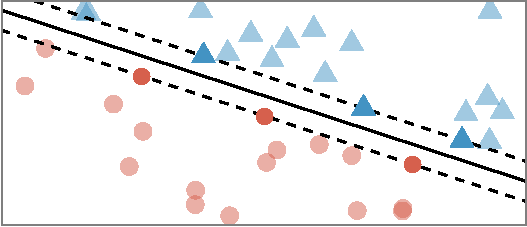
\includegraphics[width=.7\textwidth]{svmIntro}
	\caption{SVM Illustration}
	\label{fig:svmIntro}
\end{figure}
\FloatBarrier

In this example, the optimal separating hyperplane is designated by the solid line and the margins the dashed line. The points which fall on the boundaries are called support vectors, these are designated by a darker shade of red and blue. Having found this hyperplane for a given set of features enables us to then easily classify new observations based on their features. Using this process we can quickly and objectively classify country-year regime types for which labels do not already exist.

\section{Research Design}

To highlight the feasibility and gauge the performance of this classification approach, we split our sample of existing labeled data into training and test sets. For the democracy model, we have ``ground truth'' data from Polity through 2013, so we set 1999-2008 (n = 1,557) as the training set and 2009-2013 (n = 707) the test set. For the three authoritarian archetypes, we only have ``ground truth'' data from GWF and HT through 2010, so we made 1999-2006 (n = 1,138) the training set and 2007-2010 (n = 583) the test set. 

The vector space representations of our textual data are obtained from the FH and State Department reports, and we process them using the steps described earlier. One additional step that is necessary to undertake involves determining whether the features represented in the vector space models should be composed of single words (unigrams) or phrases (n-grams). We tested a number of strategies and found that the highest performance in classifying the party and military labels came from using unigrams; for monarchy, from n-grams that vary in range from one to three; and for democracy, from n-grams that vary in range from two to four.\footnote{This leads to high dimensional representations for the textual data associated with each gram choice. The number of features when using unigrams is equal to almost 25 thousand, whereas the number of features using either of the n-gram approaches surpasses one million.}

\section{Results}

The heat-map in Figure \ref{fig:aggPerf} summarizes the performance of the classifiers across our variables of interest in the out of sample test periods. The top two rows of this matrix designate the accuracy and F-1 scores for our classifiers. Accuracy provides a measure for the overall correctness of the model and is calculated as the sum of correct classifications divided by the total number of classifications. The accuracy statistic for each of our variables of interest is greater than or equal to 98\%. 

The bottom two rows of this matrix designate the precision and recall scores for our classifiers. The numerator for both precision and recall, in the case of, for example, our monarchy variable is defined as the number of country-years classified as monarchy that were also coded as being a monarchy by GWF and HT. The denominator for the precision metric is the total number of country-years classified as having a monarchy, whereas the denominator for recall is the total number of country-years labeled as monarchy by GWF and HT. We achieve 100\% precision on every variable of interest except the democracy label, for which we still receive a score of 99\%. In terms of recall, we again receive scores of greater than 90\% for each of the metrics except our military label, for which our classifier receives a score of 67\%. 

%         cat Precision    Recall F-1 Score  Accuracy
% 1 Polity>=7 0.9866667 0.9579288 0.9720854 0.9759547
% 2  Monarchy 1.0000000 0.9230769 0.9600000 0.9965695
% 3     Party 1.0000000 0.9285714 0.9629630 0.9965695
% 4  Military 1.0000000 0.6666667 0.8000000 0.9948542

\begin{figure}[ht]
	\centering
	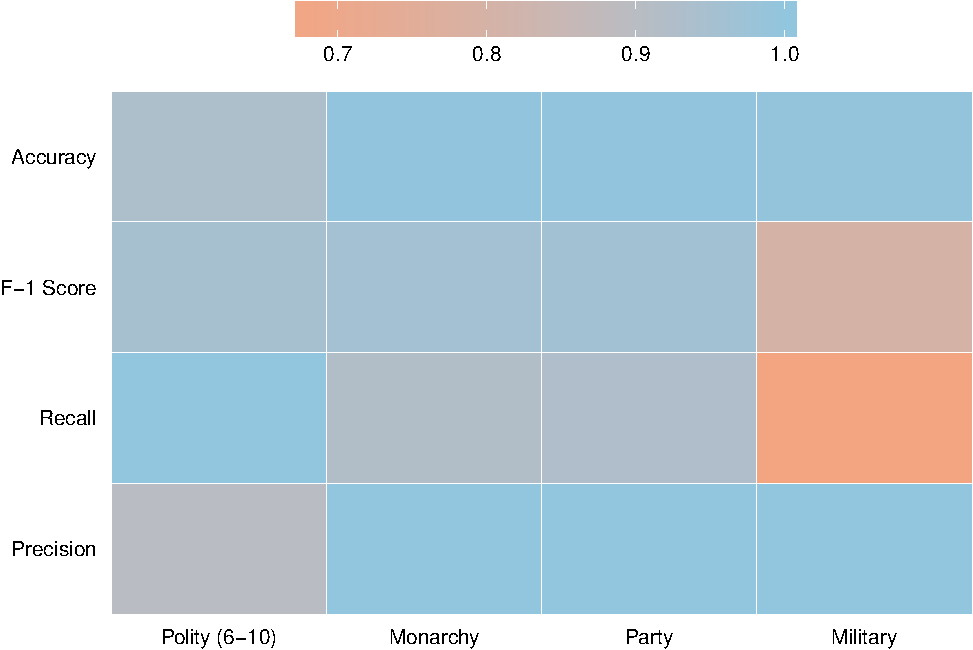
\includegraphics[width=.7\textwidth]{allAggPerf}	
	\caption{Aggregate Performance}
	\label{fig:aggPerf}
\end{figure}
\FloatBarrier

The recall metric for the military label is lower because our SVM classifier differs from the GWF and HT codings on the cases of Algeria, Pakistan, and Thailand. Figure \ref{fig:milChng} depicts the classifications received by these three countries during the test period of 2007 to 2010. The red square denotes the rating provided by GWF and HT, and the blue triangle the prediction from the SVM. In the case of Algeria and Pakistan, the difference results from the SVM classifying the countries as moving away from a militaristic regime before GWF/HT reached the same conclusion. 

\begin{figure}[ht]
	\centering
	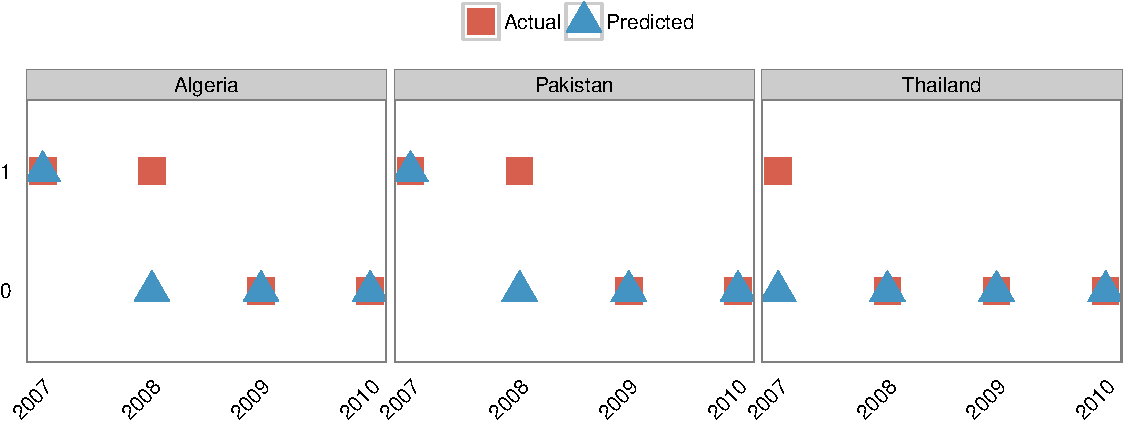
\includegraphics[width=.9\textwidth]{military_perfChange}
	\caption{Differences between SVM and GWF/HT classifications of militaristic regimes.}
	\label{fig:milChng}
\end{figure}
\FloatBarrier

Figure \ref{fig:wrdCloud} highlights a number of the features that were used by the SVMs to classify country-years into our four measures of regime type. Blue words in each word cloud represent features that made it more likely for a country-year to be classified into a regime type, while red words indicate features that made it less likely. The size of words correspond to the relative importance of that feature in the model. As we would expect, phrases such as ``free fair election'' and ``right fair trial'' are associated with a greater likelihood of a country being classified as a democracy, while features such as ``royal'' and ``king'' increase the likelihood of a country being classified as a monarchy. 

\begin{figure}[ht]
	\centering
	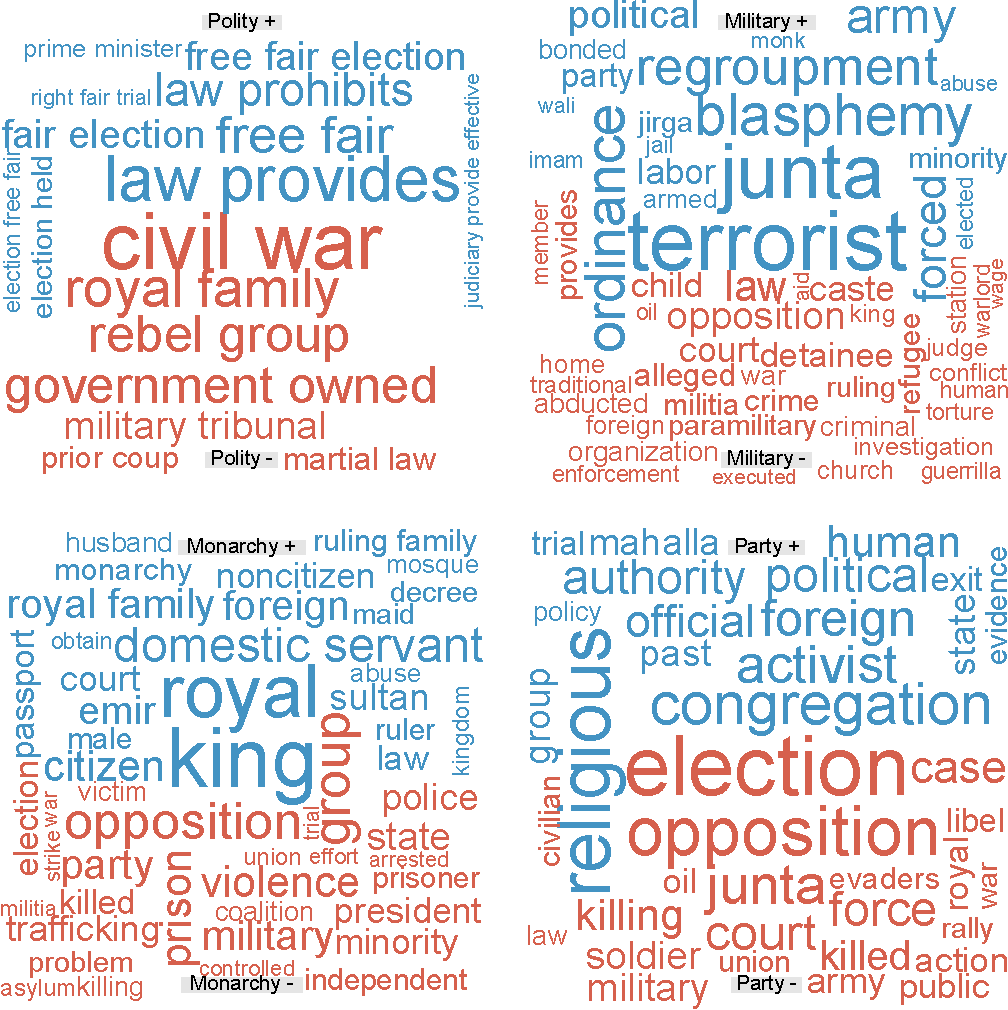
\includegraphics[width=.7\textwidth]{pol_bin_wrdCloud}
	\caption{Features used by SVM to classify country-years.}
	\label{fig:wrdCloud}
\end{figure}
\FloatBarrier

The results we have shown so far highlight that the predictions from our classifiers match well against how country-years in our test set are labeled. For each prediction in our test set, we can also calculate a ``confidence score''. These scores represent the signed distance of a particular country-year observation from the hyperplane. Distances less than zero correspond to the cases in which the classifier designates an observation as not belonging to a particular label, while scores greater than zero indicate that the observation does belong to that label. Figure \ref{fig:confDist} summarizes the out-of-sample confidence score distributions for each of the four regime types. The score distributions for the monarchy, party, and military regime types show that cases not falling into those labels are a noticeable distance away from the boundary of zero, indicating a greater level of confidence in the classification of those cases.

\begin{figure}[ht]
	\centering
	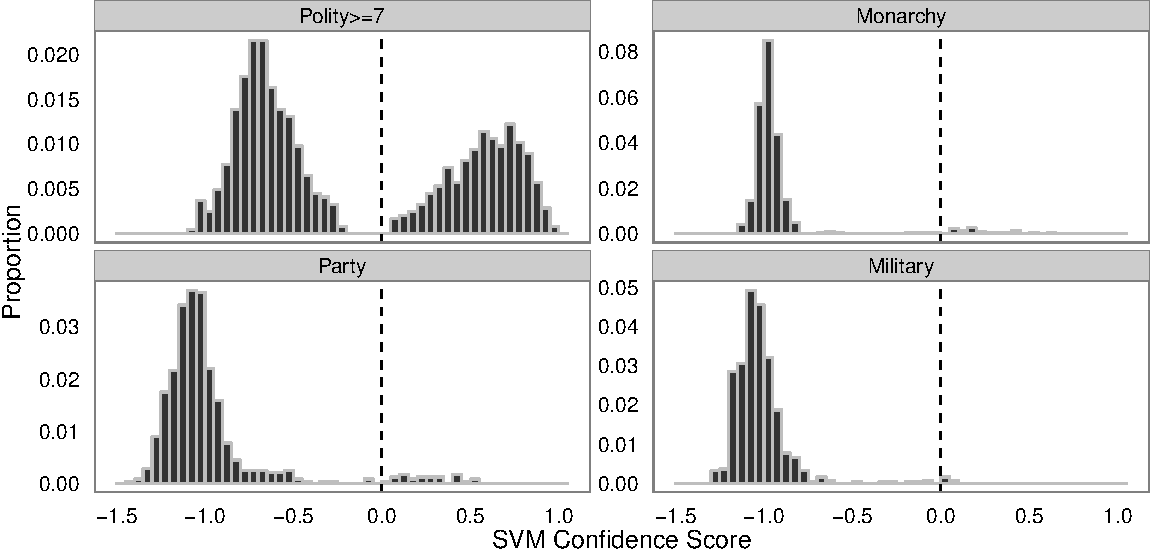
\includegraphics[width=1\textwidth]{pol_bin_probDist}
	\caption{Histograms of Out-of-Sample Estimated Confidence Scores of Four Regime Types from Support Vector Machines (SVM)}
	\label{fig:confDist}
\end{figure}
\FloatBarrier

Figure \ref{fig:confMap}, on the following page, shows variance in the SVM confidence scores for all four regime dimensions in 2009. On the whole, cases fall out as we would expect them to. The results seem valid on their face. For example, the democracy classifier confidently identifies Western Europe, Canada, Australia, and New Zealand as democracies; shows interesting variations in Eastern Europe, Latin America, and South Asia; and confidently identifies nearly all of the rest of the world as non-democracies. Meanwhile, the monarchy model correctly identifies most of the countries of the Arabian Peninsula, Jordan, and Morocco as monarchies and the rest of the world as not. The military rule classifier sees Myanmar, Pakistan, and Algeria as likely cases in 2010 and is less certain about the absence of military rule in several West African and Middle Eastern countries than in the rest of the world. Last, the map of results from the one-party rule classifier correctly identifies countries such as China, Laos, Vietnam, Turkmenistan, and Uzbekistan as instances of one-party rule but mistakenly excludes North Korea from this list in 2009.\footnote{North Korea is correctly identified as having a party based regime type in other years.} 

\begin{figure}[!t]
	\begin{tabular}{ll}
	    \hspace{-7mm}
		\subfloat[][Polity (7--10)]{
			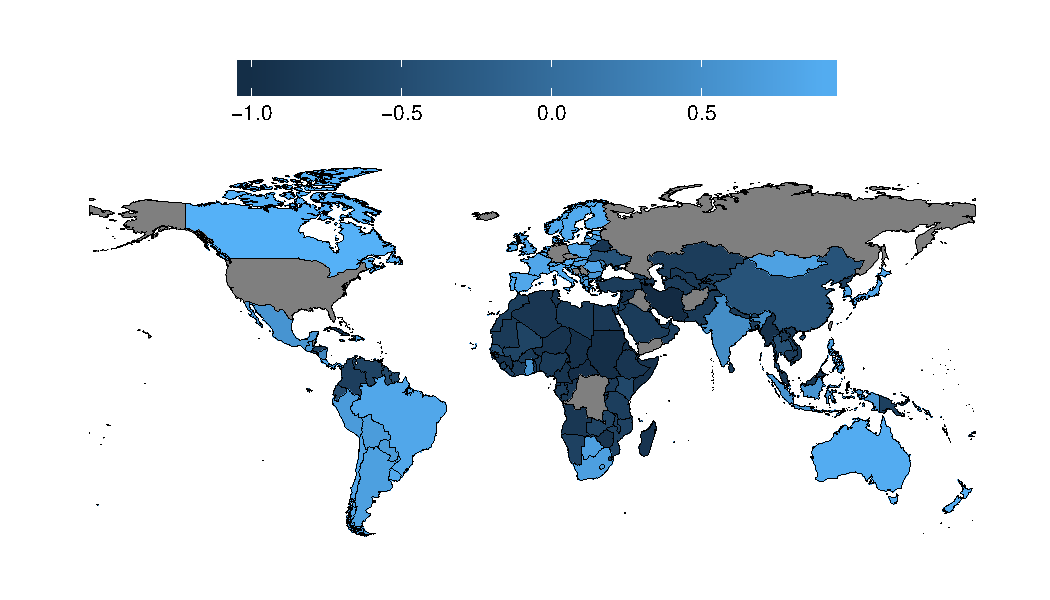
\includegraphics[width=.5\textwidth]{polGe7_2009_map}
			\label{fig:mapp4}} &
		\subfloat[][Military]{
			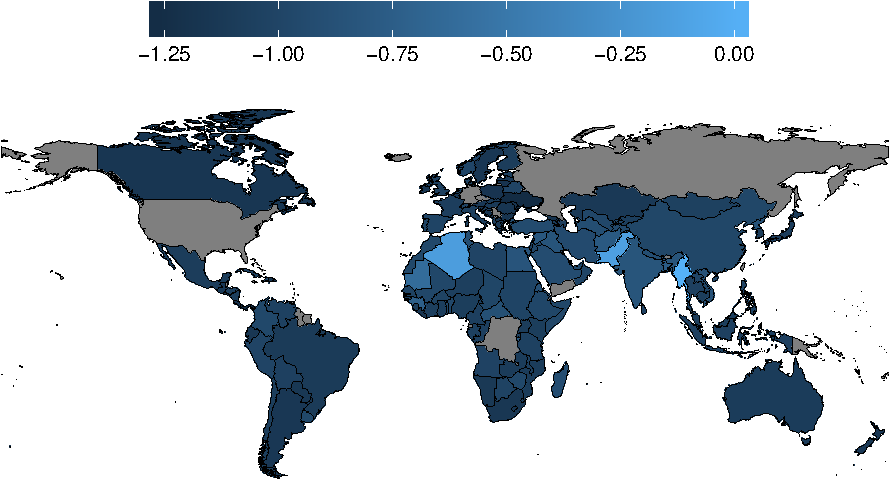
\includegraphics[width=.5\textwidth]{military_2009_map}
			\label{fig:mapmil}} \\
	    \hspace{-7mm}
		\subfloat[][Monarchy]{
			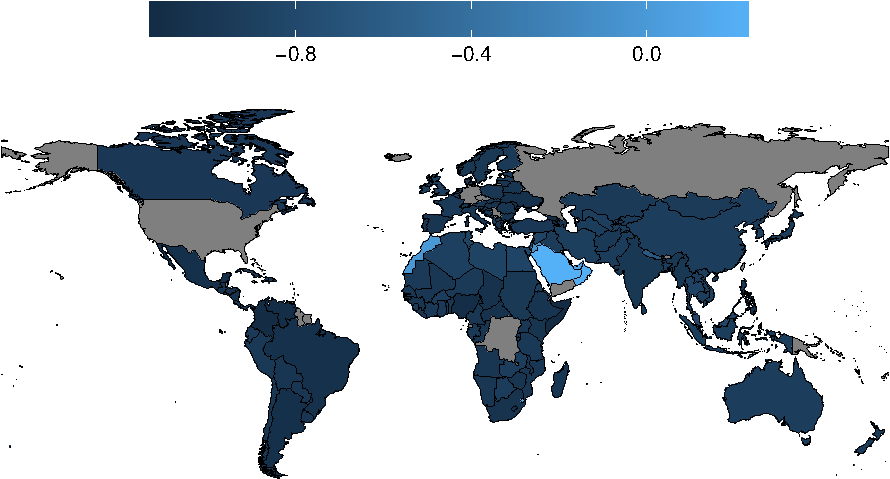
\includegraphics[width=.5\textwidth]{monarchy_2009_map}
			\label{fig:mapmon}} &
		\subfloat[][Party]{
			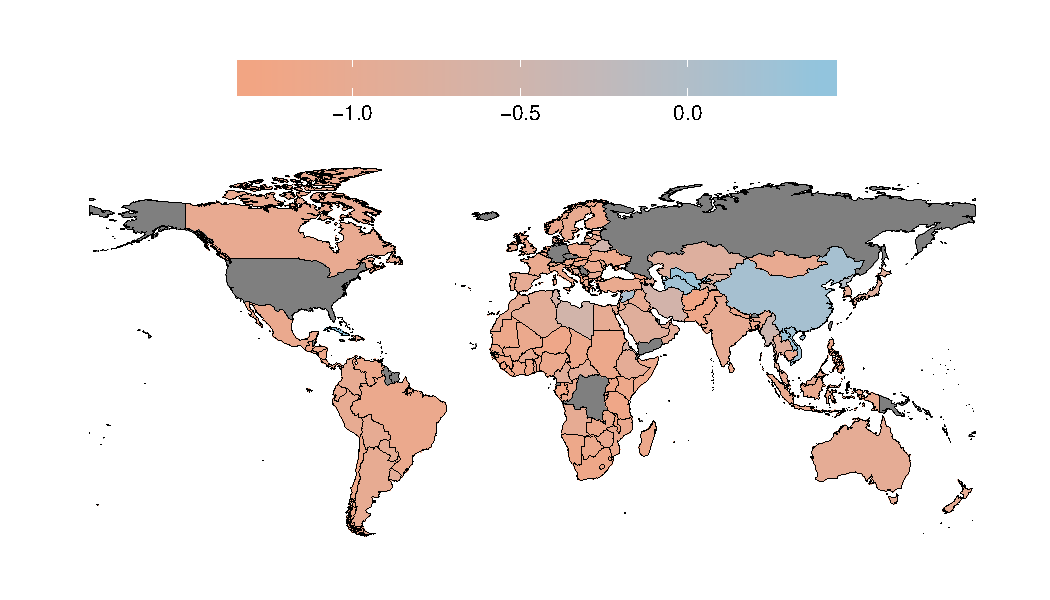
\includegraphics[width=.5\textwidth]{party_2009_map}
			\label{fig:mapparty}}
	\end{tabular}
\caption{Heat Maps of Out-of-Sample Confidence Scores from Support Vector Machines (SVM) of Four Regime Types.}
\label{fig:confMap}
\end{figure}
\FloatBarrier

\section{Conclusion}

The results described here demonstrate that it is possible to generate measures of political regime type from publicly available texts at low cost. Our initial application using features derived from a small corpus produced out-of-sample estimates that closely match observed data on several very different regime types.

Although the out-of-sample classification accuracy of our models is very good, we feel that we can improve this output by incorporating a larger sample of texts. The State Department and Freedom House texts used so far cover a narrow set of human-rights practices and political procedures. These practices and procedures are all fundamental to how we conceive and observe political regime type, but they are not the only essential characteristics.

In future iterations, we plan to expand the corpus to include annual or occasional reports that discuss a broader range of features in each country's national politics. Eventually, we hope to add news stories to the mix. If we can develop models that perform well on an amalgamation of occasional reports and news stories, we will be able to implement this process in near-real time, constantly updating measures of regime type for all countries of the world at very low cost. Making this task easier, however, will be the already created pipeline that we have set up for processing texts and generating measures of regime type. 

\newpage
\bibliographystyle{apsr}
\bibliography{MADCOWregime}

\end{document}
\bye
